\documentclass[10pt,a4paper]{article}
\usepackage[utf8]{inputenc}
\usepackage{amsmath}
\usepackage{amsfonts}
\usepackage{mathtools}
\usepackage{amssymb}
\usepackage{graphicx}
\usepackage{subcaption}
\usepackage{dsfont}
\usepackage[strict]{changepage}
\usepackage{float}
\usepackage{graphicx}
\usepackage{parskip}
\usepackage{gensymb}
\makeatletter
\newcommand*{\transpose}{%
  {\mathpalette\@transpose{}}%
}
\newcommand*{\@transpose}[2]{%
  % #1: math style
  % #2: unused
  \raisebox{\depth}{$\m@th#1\intercal$}%
}

\author{Adam Jalkemo \texttt{adam@jalkemo.se} \and
Alexander Israelsson \texttt{israelsson.alexander@gmail.com} \and
Emil Westenius \texttt{emil@westenius.se} \and
Jonathan Andersson \texttt{mat11ja1@student.lu.se}
\and 
\\
Supervisor: Gabriel Ingeson}
\begin{document}

\title{Adaptive Friction Compensation}

\maketitle
\pagebreak
\section{Introduction}
In this project adaptive friction compensation of the Furuta pendulum process have been explored. The Furuta pendulum consists of a pendulum, that is free to rotate in the vertical plane, attached to the end of an horizontally rotating arm that can be controlled. The pendulum will be stabilized in the inverted position using a swing up controller and a top controller. When controlling the pendulum in the top position limit cycles will occur due to friction. By compensating for the friction the pendulum will be stabilized and the limit cycles reduced. The friction will be estimated using an adaptive method. To do this a Java controller and interface is implemented and ran on a linux computer.
%\begin{figure}[!htb]
%\begin{center}
%\includegraphics[width=1\textwidth]{process.png}
%\caption{The furuta pendulum in the inverted position}
%\label{fig:process}
%\end{center}
%\end{figure}
\section{Program structure}
For our suggested solution we will need one thread for the GUI and one for the controller. To communicate with the Furuta process we will use the analog box normally used during the control labs at LTH. The realtime package from Automatic Control at LTH will be used for communication in the GUI and controller implementation. It will be important to synchronize the controller calculations with the user inputs. A general overview can be seen in figure \ref{fig:uml}.

\begin{figure}[!htb]
\centering
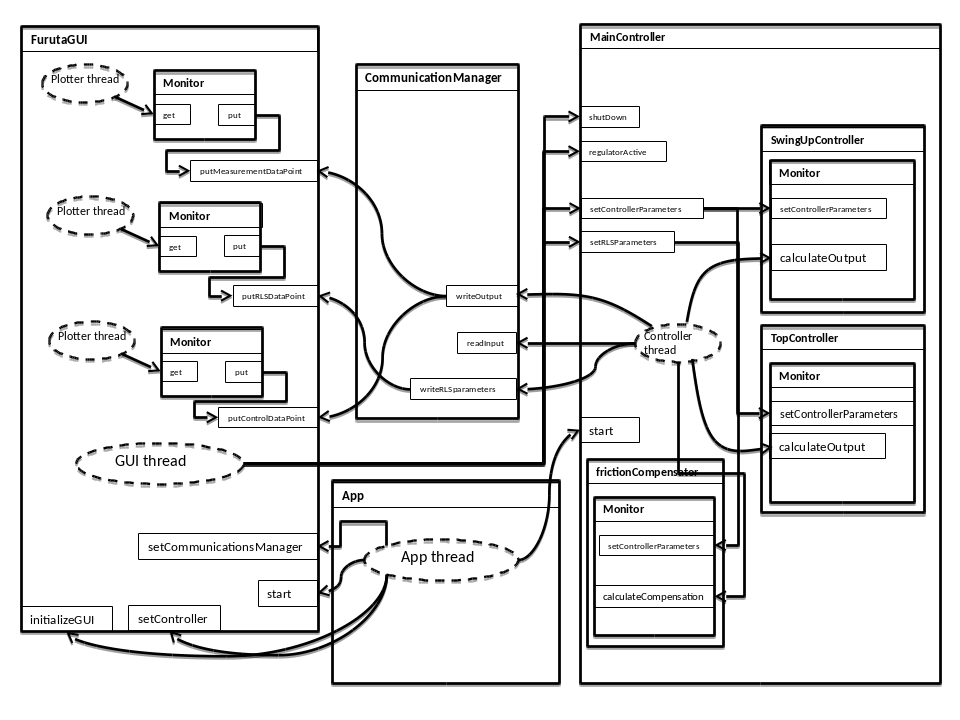
\includegraphics[width=1\textwidth]{notUml.png}
\caption{Overview of the program structure}
\label{fig:uml}
\end{figure}
%% MORe STUFFS??

%ToDo UML AND DESCRIPTION OF CLASSES AND PACKAGES

The program has three main parts: MainController, FurutaGUI and CommunicationManager. The MainController has all the control logic parts. This includes the main control loop, object for top control, object for swingup control and an object for friction compensation. The CommunicationManager is responsible for reading and passing around all the data. It reads the output from the process and fixes the scaling and offset. SpecificTests is an additional class which runs tests on the process and then saves the results to files. The Discretizer class is used for the LQR parameter calculations.

The program has two main threads, the controller and the GUI. The GUI in turn has additional threads to continously update the plot windows. The controller has higher priority than the GUI threads. Since there are only two threads that access the same shared resources and only one lock active at a time there can be no deadlocks.

The objects that are shared between the controller and the GUI are the parameters and the communicationManager object. The GUI has its own versions of the parameter objects. The parameters are all changed by copying the parameter objects from the GUI and set in blocks that are synchronized. The communicationManager object is in itself thread safe and no extra precautions are needed when used in the threads.


%Todo what parameters can be changed.
\section{System model}
Due to the non-linear dynamics of the rotating arm and pendulum the modelling of the process becomes complicated. A model given in Lab2 in "Non-linear control" has been used where the model have been simplified with the help of Lagrange theory. The dynamics of the model is then given by:
$$(J_p + Ml^2)(\ddot{\theta} - \dot{\varphi} ^2\sin\theta \cos\theta )+Mrl\ddot{\varphi}\cos\theta-gl(M+m/2)\sin\theta = 0 $$
\begin{equation}
Mrl\ddot{\theta}\cos\theta - Mrl\dot{\theta ^2}\sin\theta + 2(J_p + ml^2 ) \dot{\theta} \dot{\varphi}\sin\theta \cos\theta + (J+mr^2 + Mr^2 + (J_p+ml^2)\sin^2\theta)\ddot{\varphi}=u
\label{eq:model}
\end{equation}
where $\theta$ is the angle of the pendulum, $\varphi$ is the angle of the arm and $u$ is the motor torque on the arm. The states $\theta$, $\dot{\theta}$, $\varphi$ and $\dot{\varphi}$ will all be measured from the process and $u$ will be the control signal. The approximated coefficients are also taken from Lab2 and are given by:
$$l=0.413m \quad  r=0.235m$$
$$M=0.01kg \quad J=0.05kgm^2$$
$$J_p=0.0009kgm^2 \quad m=0.02kg$$
$$ g=9.8$$
Where $l$ is the length of the pendulum, $r$ is the length of the arm, $M$ is the mass of the weight, $J$ is moment of inertia  for pendulum, $J_p$ is the moment of inertia for the arm, $m$ is the mass of the pendulum and $g$ is the gravity constant.
\subsection{Linearization}
The model in \ref{eq:model} is then linearized around
\begin{equation}
x =
\begin{pmatrix}
\theta & \dot\theta & \varphi & \dot\varphi
\end{pmatrix} = 
\begin{pmatrix}
0 & 0 & 0 & 0
\end{pmatrix}
\end{equation}
which yields 
\begin{equation}
\dot{x} = Ax + Bu =
\begin{pmatrix}
0 & 1 & 0  & 0 \\
\frac{bd}{ab-c^2} & 0 & 0 & 0 \\
0 & 0 & 0 & 1 \\
\frac{-cd}{ab-c^2} & 0 & 0 & 0
\end{pmatrix}x
+
\begin{pmatrix}
0 \\
\frac{-cg}{ab-c^2} \\
0 \\
\frac{ag}{ab-c^2}
\end{pmatrix}u
\label{eq:linear}
\end{equation}
where 
$$ a = J_p + M l^2 \qquad b = J + M r^2 + m r^2 $$
$$ c = M r l  \qquad d = l g (M + m/2) $$
This corresponds to the arm fixed at an angle corresponding to zero and the pendulum fixed in the top position. It is in this position that the friction will create oscillations and where the adaptive friction compensation will be applied.
\subsection{Discretization}
The linearized model should preferably be discretized using ZoH. However, instead of ZoH a bilinear transformation is used in Java as an approximation of $\Phi$ since exponential matrix was not available in our matrix package. This allows the change of sampling time online. $ \Gamma $ is approximated using the approximation B*h, this is not a perfect approximation but we've not notices any major losses compared to using the ZoH discretized matrices. For the most part a sample time of $h=0.01$ have been used since this suited the system best. With $h=0.01$ the ZoH discretization of the model yields in 
% adam todo N�mner vi analoga filter osv?
% We would like to implement a way to change the sampling time online but this would require us to implement a function similar to $c2d$ in java. There are approximations that can be made so that we won't have to solve the integral over the matrix exponential but we need to be sure that the results are good enough. If we can't figure out a way to make a java implementation of $c2d$, we will discretize offline using matlab with the sample time $h=0.01$.
%This yields
\begin{equation}
x_{k+1} = A_dx_k + B_du_k =\begin{pmatrix}
 1.0016 & 0.01 & 0 & 0 \\
 0.3133 & 1.0016 & 0 & 0 \\
 0 & 0 & 1 & 0.01 \\
 -0.0059 & 0 & 0 & 1 
\end{pmatrix}x_k + \begin{pmatrix}
-0.0036\\
-0.7127\\
 0.0096\\
 1.9125
 \end{pmatrix}u_k
\end{equation}

And with the approximation described above
\begin{equation}
x_{k+1} = A_dx_k + B_du_k =\begin{pmatrix}
1.0016 & 0.01 & 0 & 0 \\
0.3134 & 1.0016 & 0 & 0 \\
0 & 0 & 1 & 0.01 \\
-0.0059 & 0 & 0 & 1
\end{pmatrix}x_k + \begin{pmatrix}
0\\
-0.7123\\
 0\\
 1.9125
 \end{pmatrix}u_k
 \label{eq:discrete}
\end{equation}

\section{Controller}
There are six measurement signal available for the controllers to use. Two for the position $ \theta $ and velocity $ \dot{\theta} $ of the pendulum each (one has higher resolution and can only  be used at the top position) and one for the arm position $ \varphi $ and velocity $ \dot{\varphi} $. Monitoring the signals there was no noticeable difference between the higher resolution and $ 360 \degree $-sensor and we therefore only used the two measurements from the $ 360 \degree $ sensor.
\subsection{Swing up}
For the swing up of the pendulum a Lyapunov based controller is used. For the Lyapunov candidate the total energy (kinetic and potential) of the pendulum will be considered and is given by 
\begin{equation}
E= Mgl(cos\theta - 1)+\frac{J_p}{2}\dot\theta^2
\label{eq:energy}
\end{equation}
The Lyapunov candidate is then chosen as $V(x,a)=E^2$. By then taking the derivative of the candidate a controller $a=F(x)$ is derived which will make $\dot V \leq 0$ for all $x$. The controller will always output the maximal control signal possible in order to minimize the Lyapunov function.
\subsection{Top controller}
In the top position a LQR controller is used. For this the linearized model in eq. \ref{eq:linear} is used to calculate L. In order to change the cost of matrices Q and R online a way to calculate the state feedback gain vector L was implemented and given by
$$ L = (R+B^TPB)^{-1}(B^TPA) $$
where P is calculated by iterating
$$ P_{k-1} = A^TP_kA-(A^TP_kB)(R+B^TP_kB)^{-1}(B^TP_kA)+Q $$
backwards in time with $P_N = Q$. This solution for the Riccati problem will not work for all systems but in this case Fredrik Bagge verified that it should work.

To remove remaining error in $\phi$ an integral action is introduced. The error is simply integrated and multiplied by an adjustable gain and then added to the control signal. Anti-Windup is done with a resetting factor.
% todo write about integral action

\subsection{Controller switch}
In order to switch between the two controllers good conditions is necessary to enable the pendulum to be in a good position for when the top controller takes over. Since the model is linearized around 
$$x =
\begin{pmatrix}
\theta & \dot\theta & \varphi & \dot\varphi
\end{pmatrix} = 
\begin{pmatrix}
0 & 0 & 0 & 0
\end{pmatrix}$$
the pendulum needs to have both a low velocity and be close to the top for the top controller to work properly. The switching conditions is chosen as an ellipse made from $\dot\theta$ and $\theta$ which will give good estimations of when to switch. Since $ \varphi $ might be far from zero one might run into troubles if this in punished heavily. We solve this by resetting $ \varphi $ when the top controller takes over.


\section{Friction compensation}
When controlling the pendulum in the top position there will be limit cycles due to the friction. To minimize these cycles RLS based friction compensation is added to the top controller. When the pendulum is close to the top position a dead-zone is added in order to keep the noise from the measurements from making the friction compensation add control signal in the wrong direction. There are a lot of different ways to model friction. Some really complicated and some pretty simple. In fig \ref{fig:fric} measured friction of the process can be seen for different velocities. The oscillating behaviour is believed to be due to different friction in different directions. Since the average friction for the different velocities did not vary that much and the measured signals are noisy the models of the frictions were kept simple. The models used can be seen in fig \ref{fig:frictmodel}. 

%When the This will only be used in the top controller since the swing up controller will always output maximal control signal. When the pendulum is close to the top position we will need to add a dead-zone in order to keep the noise from the measurements from making the friction compensation add control signal in the wrong direction.
\begin{figure}[!htb]
\centering
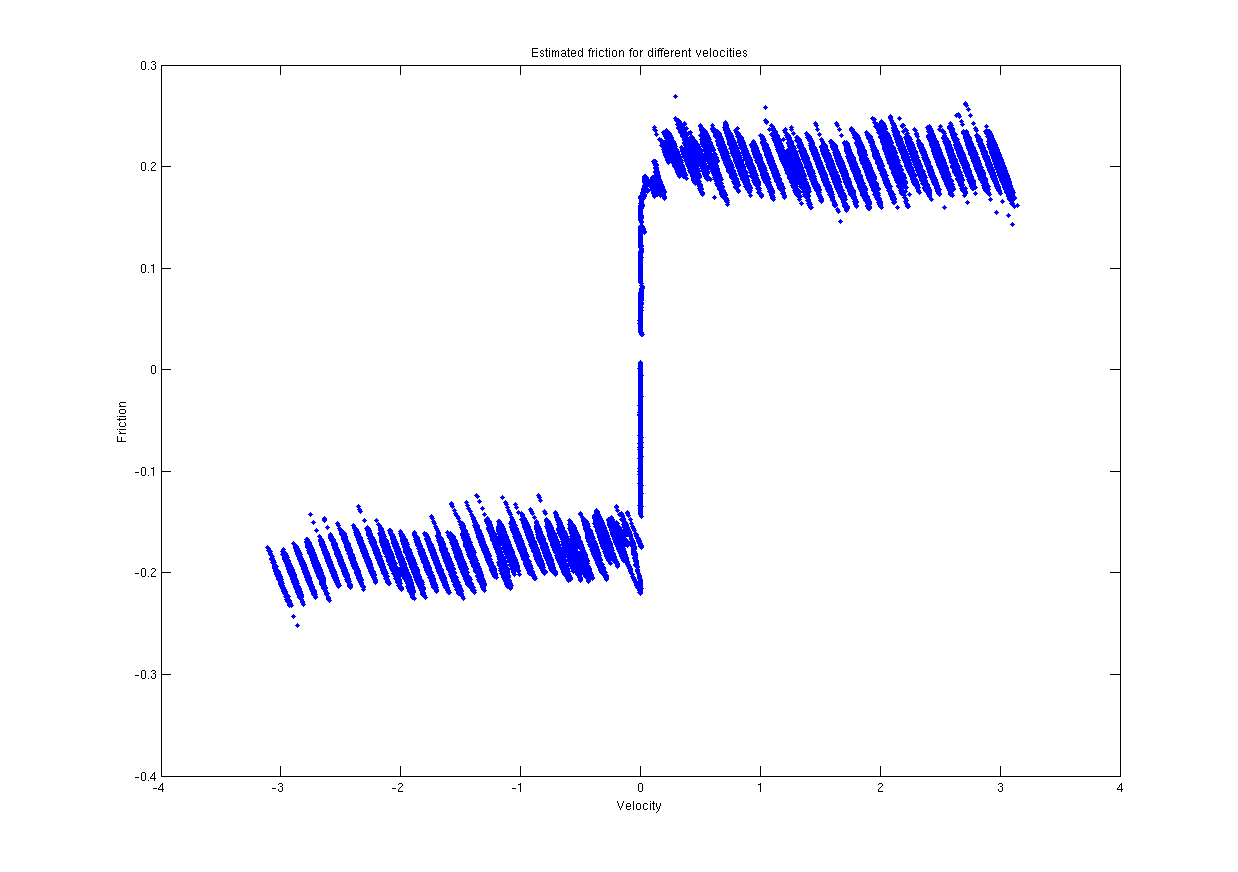
\includegraphics[width=1\textwidth]{fric.png}
\caption{Measured friction of the process for different velocities}
\label{fig:fric}
\end{figure}
\begin{figure}[!htb]
\centering
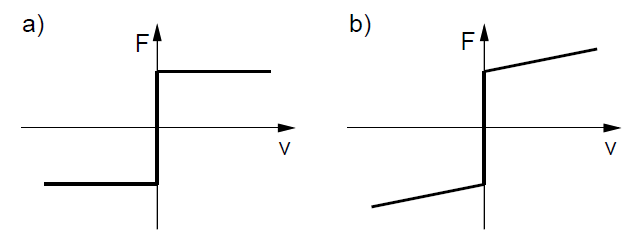
\includegraphics[width=1\textwidth]{frictmodel.png}
\caption{a) Friction model with coulomb friction. b) Friction model with coulomb and viscous friction.}
\label{fig:frictmodel}
\end{figure}
\subsection{Friction estimation}
\label{sec:fricEst}
To manage the friction an estimate of a simple friction model is derived using RLS. The models in fig \ref{fig:frictmodel} will respectively give the following friction expressions 
\begin{equation}
 f=f_c\cdot sign(\dot{\varphi})
 \label{eq:f}
 \end{equation}
\begin{equation}
 f=f_c\cdot sign(\dot{\varphi})+f_v\cdot \dot{\varphi}
 \label{eq:fv}
 \end{equation}
where \ref{eq:f} is model a and only depends on the direction of the velocities and \ref{eq:fv} is the model in b where a viscous term that depends on the velocity is added.
 
The regression models for the two friction models will take the form of \ref{eq:regressora} and \ref{eq:regressorb} respectively.
\begin{equation}
\phi=sign(\dot{\varphi}), \beta = f_c
\label{eq:regressora}
\end{equation}
\begin{equation}
\phi=\begin{bmatrix}
sign(\dot{\varphi}) \\
\dot{\varphi}
\end{bmatrix}, \beta = \begin{bmatrix}
f_c\\
f_v
\end{bmatrix}
\label{eq:regressorb}
\end{equation}
Since the friction can be seen as a direct negative torque on the arm, it can be directly subtracted from the control signal which gives us the system in \ref{eq:discrete}
%$$x_{k+1} = A_dx_k + B_d(u_k - f)$$
%To get the RLS to work we take all measurements one step back in time and try to estimate the parameters from \ref{eq:regressorb}. We also aim to use the measurement from the arm velocity where we get values from both the pendulum position and the arm velocity, see the state equation for $ \varphi $  in eq. \ref{eq:discrete}. After placing all known variables on the left hand side and we the following

\begin{equation}
 x_{k+1} = A_dx_k + B_d(u_k - f)
\label{eq:modwf}
\end{equation}
To get the RLS to work all measurements are taken one step back in time to estimate the parameters from \ref{eq:regressora} or \ref{eq:regressorb}. After rearranging the equation in \ref{eq:modwf} we get
\begin{equation}
 \dfrac{x_{k}-A_dx_{k-1}-B_d u_{k-1}}{-B_d} =   f
\label{eq:estim}
\end{equation}
%\frac{\dot{\varphi}_k + 0.0059\theta_{k-1}-1.9125u_{k-1}-\dot{\varphi}_{k-1}}{-1.9125} = \begin{pmatrix}
%f_c & f_v
%\end{pmatrix}\begin{pmatrix}
%\dot{\varphi}_{k-1}\\
%sign(\dot{\varphi})
%\end{pmatrix}

where $f$ is one of the regressors in \ref{eq:regressora} or \ref{eq:regressorb}. By choosing one of the states in $x$ the normal RLS algorithm can be applied with some forgetting factor $\lambda$, the algorithm is given in \ref{subsec:rlsalg}.
\\
Since the friction of the process have different friction for different directions of the arm, some trials with an extra state in the regressors was also done. The extra state was added to the regressors as a constant to offset the imbalance of the friction compensation for the different directions. The regressors are then given by 
\begin{equation}
\phi=\begin{bmatrix}
sign(\dot{\varphi}) \\
1
\end{bmatrix}, \beta = \begin{bmatrix}
f_c\\
f_o
\end{bmatrix}
\label{eq:regressorao}
\end{equation}
\begin{equation}
\phi=\begin{bmatrix}
sign(\dot{\varphi}) \\
\dot{\varphi} \\
1
\end{bmatrix}, \beta = \begin{bmatrix}
f_c\\
f_v\\
f_o
\end{bmatrix}
\label{eq:regressorbo}
\end{equation} 

%As we see in equation \ref{eq:discrete} we probably can get different results in the friction estimation by choosing different equations in the same form as in equation \ref{eq:estim}. Initially we want to estimate the friction when the pendulum is hanging straight down and the arm is rotating at a constant speed. If there were no friction, no control signal would be necessary to keep the velocity of the arm constant, and therefore the control signal required corresponds to the signal necessary for compensating the coloumb friction.
%We also want to to estimate the friction in the top position and then the equation corresponding to the state $ \dot{\varphi} $ in eq. \ref{eq:discrete} might not be the one which yields the best result. More research will be put into this at a later stage.

% More research at a later stage??

\subsection{Recursive least squares algorithm}
\label{subsec:rlsalg}
To estimate the parameters throughout this project the standard recursive least squares algorithm with a added forgetting factor will be used as stated below. 
\begin{equation}
\hat{\theta}_k = \hat{\theta}_{k-1}+P_k\phi_k\epsilon_k 
\end{equation}
\begin{equation}
\epsilon_k=y_k-\phi_k^{T}\hat{\theta}_{k-1} 
\end{equation}
\begin{equation}
P_k=\frac{1}{\lambda}(P_{k-1}-\frac{P_{k-1}\phi_k\phi_k^{T}P_{k-1}}{\lambda+\phi_k^{T}P_{k-1}\phi_k})
\end{equation}
Above $\hat{\theta}_k$ is the estimated parameters , $\phi_k$ is the regressor, $P_k$ is a matrix is the estimate of the parameter covariance and $\lambda$ is the forgetting factor.

\section{GUI}
The operator is able to change parameters for both controllers and for the friction estimator.

For the top controller, the $Q$ and $R$ matrices and the integrating factor can be changed. For the swing up controller, the "switching area", natural frequency and gain can be changed. Other general parameters for the controller such as sampling time $h$ and deadzones can also be changed.

For the friction estimation the forgetting factor $\lambda$ and the initial values of $\omega _0$ can be changed. One can also switch between the three available friction models (Coloumb friction, viscous friction and viscous friction with offset). At the top right of the GUI one can enable or disable the friction compensation.

In order to save data to file buttons have been added to start and stop this process (MATLAB .mat files are stored to the root folder of the java project). There are also tests for running step responses and for running a test of the RLS convergence (without manual excitation). Both tests automatically stores the data. 

The GUI will plot the outputs from the Furuta pendulum, the friction estimation and the control signal.

See figure \ref{fig:gui} for an image of the GUI.

% TODO UPDATE IMAGE
\begin{figure}[!htb]
\begin{center}
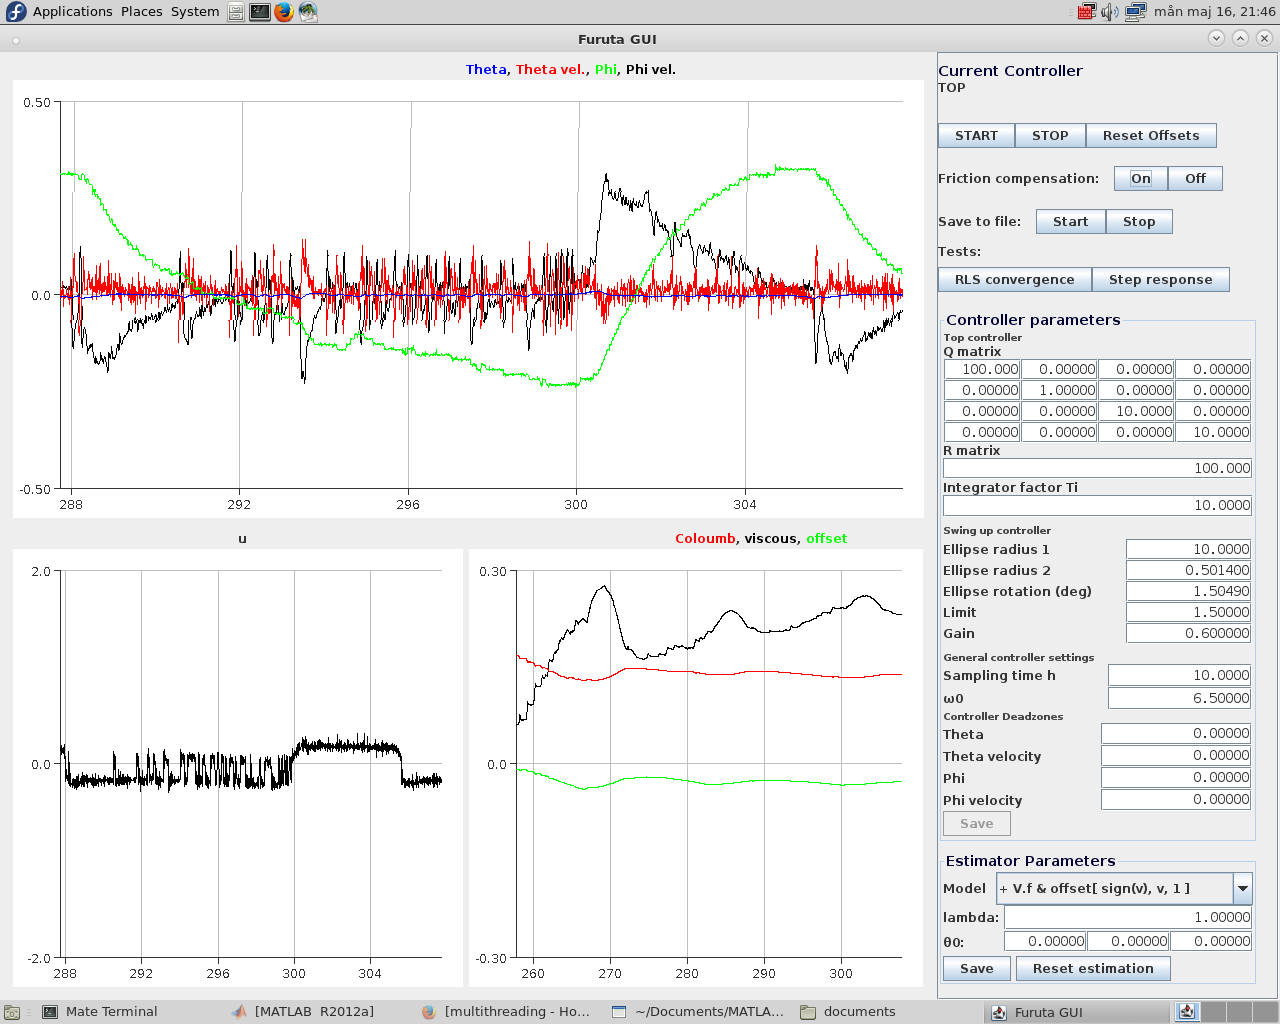
\includegraphics[width=1\textwidth]{gui.png}
\caption{Overview of the program structure}
\label{fig:gui}
\end{center}
\end{figure}
\section{Results}


\subsection{Limit cycles}
The limit cycles of the system got significantly lower when adding the friction compensation using the estimated parameters of the friction. The behaviour of the arm angle and pendulum angle can be viewed in \ref{fig:onoffcompensation} where \ref{eq:regressorb} was used as a friction model.
\begin{figure}[H]
\begin{center}
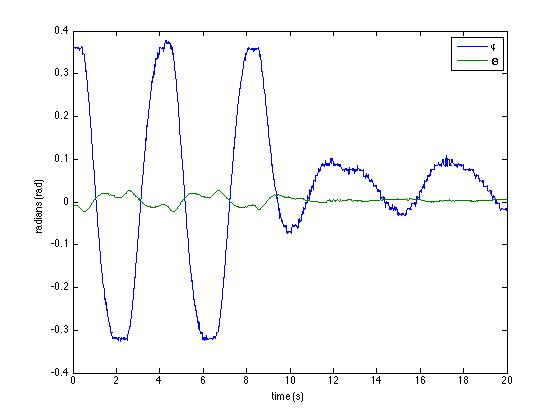
\includegraphics[width=1\textwidth]{plots/onoffcompensation.jpg}
\caption{Arm and pendulum angle behaviour in steady state and turning on friction compensation after 10 seconds. The parameter estimation, after manual excitation of the system, converged before being turned on.}
\label{fig:onoffcompensation}
\end{center}
\end{figure}
In \ref{fig:onoffcompensation} see that the amplitude of the limit cycles are lowered to about a third of the size. We can also see an offset from the zero angle.
\subsection{Coloumb + viscouse friction model}
In \ref{fig:srvisc} we can see the behaviour of the angle and angular velocity for both the arm and the pendulum.
\begin{figure}[H]
\centering
		\begin{subfigure}[t]{0.49\textwidth}
			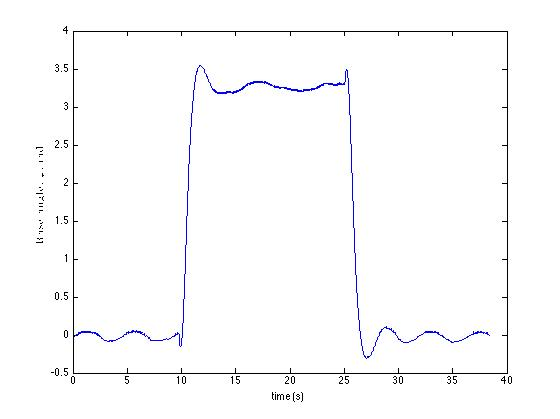
\includegraphics[scale=0.33]{plots/steprespviscphi.jpg}
			\centering
			\caption{The step response for the angle of the arm.}
			\label{subfigure:srviscphi}
		\end{subfigure}
		\begin{subfigure}[t]{0.49\textwidth}
			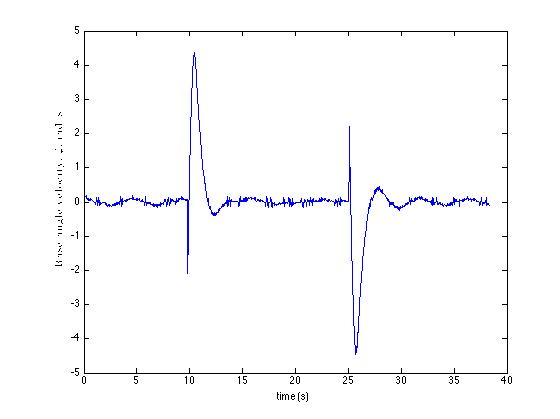
\includegraphics[scale=0.33]{plots/steprespviscphidot.jpg}
			\centering
			\caption{The step response for the angular velocity of the arm.}
			\label{subfigure:srviscphidot}
		\end{subfigure}
		\begin{subfigure}[t]{0.49\textwidth}
			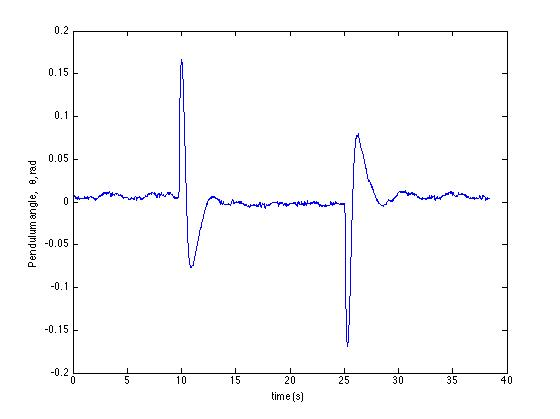
\includegraphics[scale=0.33]{plots/steprespvisctheta.jpg}
			\centering
			\caption{The step response for the angle of the arm.}			
			\label{subfigure:srvisctheta}
		\end{subfigure}
		\begin{subfigure}[t]{0.49\textwidth}
			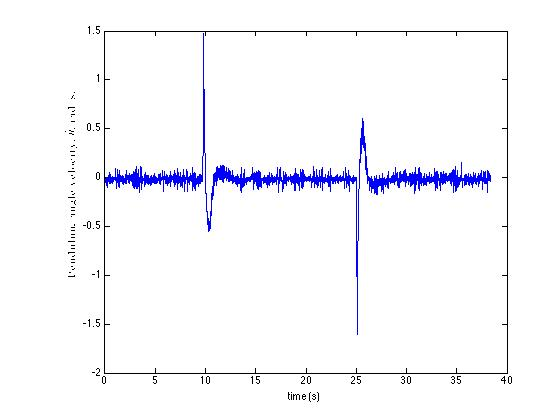
\includegraphics[scale=0.33]{plots/steprespviscthetadot.jpg}
			\centering
			\caption{The step response for the angular velocity of the pendulum.}						
			\label{subfigure:srviscthetadot}
		\end{subfigure}
		\caption{Stepresonses for the pendulum and arm positions and velocities for the using the coloumb+viscouse friction model.}
		\label{fig:srvisc}
\end{figure}
\subsection{Friction estimation}
In figure \ref{subfigure:VLUFcol} and \ref{subfigure:VLUFvisc} the calculated fricion and the calculated compensation signal is presented for both the coloumb and the coloumb+viscouse friction models.
\begin{figure}[H]
\centering
	\begin{subfigure}[t]{0.49\textwidth}
	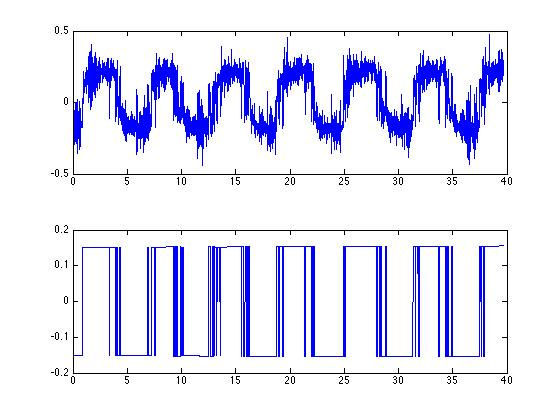
\includegraphics[width=1\textwidth]{plots/VLUFcol.jpg}
	\caption{The calculated friction and the calculated compensation control signal for the coloumb friction model given in eq \ref{eq:regressora}}
	\label{subfigure:VLUFcol}
	\end{subfigure}
	\begin{subfigure}[t]{0.49\textwidth}
	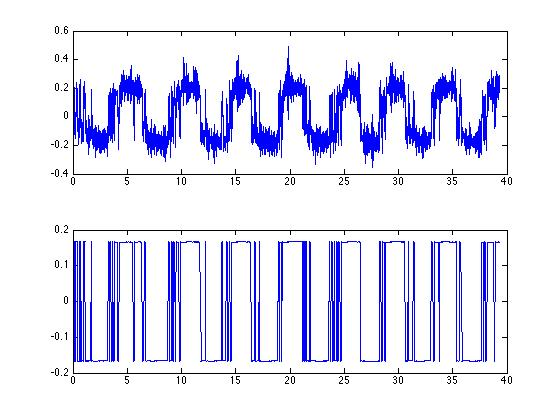
\includegraphics[width=1\textwidth]{plots/VLUFvisc.jpg}
	\caption{The calculated friction and the calculated compensation control signal for the coloumb+viscouse friction model given in eq \ref{eq:regressorb}}\
	\label{subfigure:VLUFvisc}
	\end{subfigure}
\caption{Friction calculation and estimation}
\label{fig:VLUF}
\end{figure}
\begin{figure}
\centering
%\includegraphics[width=1\textwidth]{plots/VLUFoffset.eps}
\caption{The calculated friction and the calculated compensation control signal for the coloumb+viscouse friction model with offset given in eq \ref{eq:regressorbo}}
\label{fig:VLUFoffset}
\end{figure}


\subsection{RLS estimation}
The convergence for the parameter estimation is presented in figure \ref{fig:rlsconv} both with and without external excitation.
\begin{figure}[H]
\centering
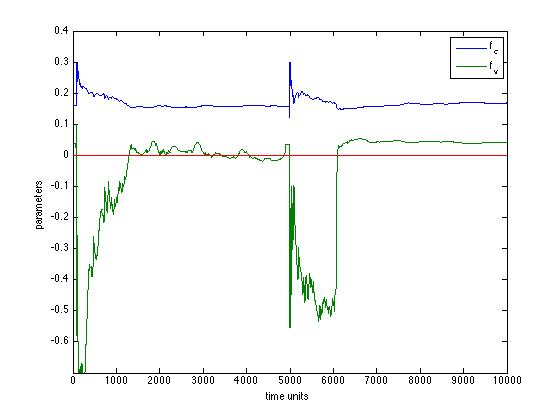
\includegraphics[width=1\textwidth]{plots/rlsconvergence.jpg}
\caption{The convergence of the friction parameters given in eq \ref{eq:regressorb}. At time t=5000 time units the estimation is reset and the system is subjected to external excitation.}
\label{fig:rlsconv}
\end{figure}
%% Fler plots
% RLS med offset
% onoffcompensation med offset
% onoffcompensation med offset och integrator
% stepresp med offset med integrator




\section{Discussion}
% Friktionsmodell, vilka det var, hur lika de va, varför vi fokuserar på col+visc
% Offset leder till utökad regressor, hjälpte inte även om observerad offset indikerade detta,
% Integrating part to remove offset in phi. Would need integrating part in theta, possible.

% Rls convergence with forgetting factor discussion


% Sticktion
% Theta offset
% Noise in thetadot and phidot due to integration
% Testade Kalmanfilter
% conclusion-can only supress limitcycles so far.
\subsection{Friction model}
A fundamental part of this project was to select a friction model for which a good compensation could be made. As stated we chose to try a coloumb friction model and and model with added viscouse part, the difference can be seen in figure \ref{fig:frictmodel}. After the results in \ref{fig:VLUF} we decided that since they were very similar we would focus on the coloumb+viscouse friction model which had a higher potential to be close to the real friction.
Since we observed that the friction is different depending on the sign of the arm velocity in \ref{fig:fric} we added a constant offset to our regressormodels, the coloumb+viscouse friction regressors with and without offset can seen in equation \ref{eq:regressorb}  and \ref{eq:regressorbo} respectively. This leads to a better representation of the friction which can be seen in figure \ref{fig:VLUFoffset}. The discrepency in the amplitude of the friction calculation is likely due to process changes, however \ref{fig:VLUFoffset} still shows the better representation of the calcluated friction.


\subsection{}
Our initial thought was that this would be the reason for the offset we can see in \ref{fig:onoffcompensation} however after adding the offset we could still observe the same behavior, see \ref{fig:onoffcompoffset}.

$ $This resulted in an improved limit cycle behavior and marginally better step responses$ $.

\subsection{RLS}
As expected the convergence for the RLS friction coefficients are a lot better with the external excitation compared to when there are no external excitation at all. Without the extra excitation the coefficients would sometimes not converge at all or even converge to negative values. With the external excitation we got a pretty fast convergence to values that would be considered reasonable for the coefficients. The external excitation was simply done by not using the compensation to begin with, resulting in the limit cycles exciting the the system enough to get a good convergence of the coefficients.\\

As for the forgetting factor we tested some different values and found that using a high value $\lambda = 0.9999$ works the best since out signals are quite noisy and there should not be any large changes to the friction or the process. 
%Forgetting factor



\section{Conclusion}






\end{document}
% Ändra alla figurer till eps??
% Bad disticntion between figure and equation, decide on norm?

%\subsection{Friction model}
%

% OTHER PART

%

%This led us to add an integrative part in order to move the arm position so it would oscilata around the true zero position, the result of adding this integrative part can be seen in \ref{fig:onoffcompintegrate}.

%As we can see the limit cycles does not dissappear completely. This can depend on a number of different factors, one major factor is likely that the offset for the pendulum position in the top position is not perfect which would lead to over- and under correction i.e. the controller will operate on position values which are not true.

% forgetting factor



